\setAuthor{Krister Kasemaa}
\setRound{piirkonnavoor}
\setYear{2022}
\setNumber{G 5}
\setDifficulty{5}
\setTopic{TODO}

\prob{Satelliittelevisioon}
Lapimaal, laiuskraadil $\varphi =\ang{67}$ elav Jussi soovib endale paigaldada satelliittelevisiooni. Satelliittelevisiooni võimaldavad satelliidid on geostatsionaarsel orbiidil. Eeldage, et satelliittelevisioon toimib, kui satelliit asub horisondist kõrgemal. Maa raadius $R=\qty{6371}{\km}$, Maa pöörlemisperiood $T=\qty{23}{\hour}\, \qty{56}{\min}$ ja raskuskiirenus maapinnal $g= \qty{9.81}{\m\per\s\squared}$.\\
\osa Kas Jussi saab endale satelliittelevisiooni paigaldada?\\
\osa Mis on suurim laiuskraad, millel on satelliittelevisiooni paigaldamine veel võimalik?
\\ \emph{Märkus}: satelliit geostatsionaarsel orbiidil on maapinna suhtes paigal.


\hint

\solu
Leiame geostatsionaarse orbiidi raadiuse. Sateliidile mõjuvad jõud on tasakaalus:
\begin{align*}
\frac{GMm}{r_\text{orbiit}^2}&=\frac{mv^2}{r_\text{orbiit}}\\
\implies \frac{GM}{r_\text{orbiit}}&= \bigg( \frac{2\pi r_\text{orbiit}}{T} \bigg)^2\\
\implies r_\text{orbiit}^3 &= T^2 \frac{GM}{4 \pi^2}.
\end{align*}
Maakera pinnal aga kehtib mingi suvalise massi $m$ jaoks:
\begin{equation*}
  \begin{cases}
    F = \frac{GMm}{R_\oplus^2}, \\
    F = mg. \\
  \end{cases}
\end{equation*}
Seega, $GM = g R_\oplus^2$. Asendades saadud seose orbiidi raadiuse valemisse, saame:
\begin{align*}
r_\mathrm{orbiit}^3 &= T^2 \frac{g R_\oplus^2}{4 \pi^2},\\
\implies r_\mathrm{orbiit} &\approx \SI{42148}{km}.
\end{align*}
Maksimaalsel sateliittelevisiooni võimaldaval laiuskraadil on sateliiti ja maakera ühendav sirge maakera puutujaks sellel maksimaalsel laiuskraadil. Seega saame seose:
\begin{figure}[h]
  \centering
  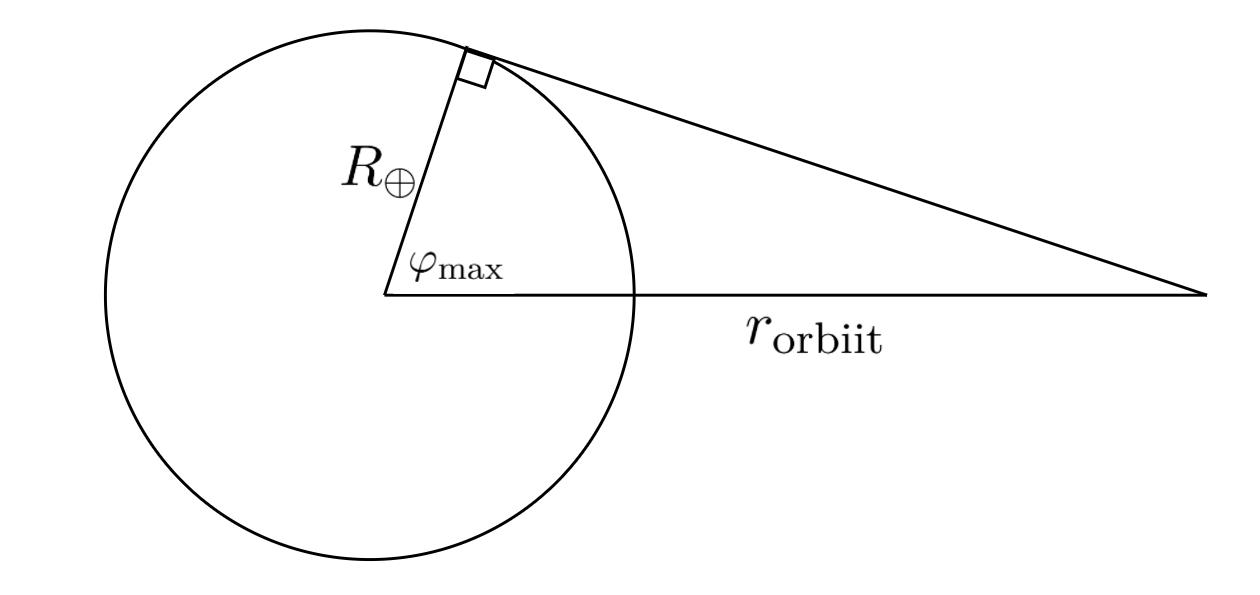
\includegraphics[width = 0.7\textwidth]{2022-v2g-05-sol.png}
\end{figure}
\begin{equation*}
\varphi_\mathrm{max} = \arccos{\left( \frac{R_\oplus}{r_\text{orbiit}}\right)} = \ang{81.3}
\end{equation*}
\probend